\documentclass[10pt,mathserif]{beamer}

\usepackage{graphicx,amsmath,amssymb,tikz,psfrag,subfigure,bm}

\input defs.tex

%% formatting

\mode<presentation>
{
\usetheme{default}
}
\setbeamertemplate{navigation symbols}{}
\usecolortheme[rgb={0,0,0}]{structure}
\setbeamertemplate{itemize subitem}{--}
\setbeamertemplate{frametitle} {
	\begin{center}
	  {\large\bf \insertframetitle}
	\end{center}
}

\AtBeginSection[] 
{ 
	\begin{frame}<beamer> 
		\frametitle{Outline} 
		\tableofcontents[currentsection,currentsubsection] 
	\end{frame} 
} 

%% begin presentation

\title{\large \bfseries Sparse linear models}

\author{Jiali Lin\\[3ex] 
        Virginia Tech}

\date{\today}

\begin{document}

\frame{
\thispagestyle{empty}
\titlepage
}

\section{Introduction}
\begin{frame}{Introduction}
    \begin{itemize}
    \item Consider a generalized linear model, $p(y|\bm{x}) = p(y|f(\bm{w}^T \bm{x}))$ for some link function $f$. 
    \item \textbf{Goal}: perform feature selection by encouraging the weight vector $\bm{w}$ to be \textbf{sparse}, i.e., to have lots of zeros.
    \item When $p$ is large, it becomes unrealistic to go through all possible choices and determine the best subset of variables based some selection criterion such as, AIC or BIC.
    \end{itemize}
\end{frame}

\section{Bayesian Variable Selection}
\begin{frame}{Bayesian Variable Selection}
    \begin{itemize}
        \item A natural way to pose the variable selection problem is to introduce a hyper-parameter $\gamma_j$ to the prior $w_j$, where 
        \begin{equation*}
          \gamma_j=\begin{cases}
            1, & \text{feature $j$ is in}\\
            0, & \text{feature $j$ is out}
          \end{cases}
        \end{equation*}
        \item We will seek various summary statistics. A natural one is the posterior mode, or \textbf{MAP} estimate
        \begin{equation*}
          \hat{\bm{\gamma}} = \argmax_{\bm{\gamma}}p(\bm{\gamma}|D) = \argmin f(\bm{\gamma})
        \end{equation*} 
        \item Drawbacks:
            \begin{itemize}
            \item Still need to search over all possible $\bm{\gamma}$.
            \item The mode of the posterior distribution does not necessarily represent the full posterior distribution well.
            \item Alternative: median of the marginal inclusion probabilities. Then we have $\hat{\bm{\gamma}} = \{j : p(\gamma_j=1|D) > .5\}$.
            \end{itemize}
    \end{itemize}
\end{frame}

\begin{frame}{Case I: Spike and slab model}
    \begin{itemize}
        \item \textbf{Main idea}: Find a prior has a mixture of a point mass at $0$ (forcing $w_j = 0$, and excluding that covariate $j$) and a flat prior (Gaussian, often) on the included variables.
        \item A common prior on the feature inclusion vector
        \begin{equation*}
            p(\bm{\gamma}|\pi_0) 
              =   \prod_{j=1}^n\text{Bern}(\gamma_j|\pi_0) 
              =   \pi_0^{\|\gamma\|_0} (1-\pi_0)^{(p - \|\gamma\|_0)}
        \end{equation*}
        \item Spike and slab prior
        \begin{equation*}
          w_j|\sigma^2,\gamma_j \sim
          \begin{cases}
            \delta_0(w_j), & \text{if $\gamma_j = 0$}\\
            N(w_j|0,\sigma^2\sigma_w^2), & \text{if $\gamma_j = 1$}
          \end{cases}
        \end{equation*}
        \item The interpretation of the two mixture components: clustering each predictor as noise (the spike at 0; excluded) and signal (the slab; included).
    \end{itemize}
\end{frame}

\begin{frame}{Case II: Bernoulli-Gaussian model}
    \begin{itemize}
        \item The prior distribution of $w_j$
        \begin{equation*}
          w_j|\gamma_j \sim \gamma_j N(0,v_{1j}^2) + (1-\gamma_j) N(0,v_{0j}^2) 
        \end{equation*}
        \item $v_{1j}$ is far from zero but $v_{0j}$ is close to zero, $v_{1j} \geq v_{0j} > 0$.
        \item This prior is a normal with variance either large or close to zero depending on the value of $\gamma_j$. 
        \item When $\gamma_j = 0$, $w_j$ has a normal prior with small variance $v_{0j}$. Since $v_{0j}$ is close to zero, $w_j$ can be a priori excluded from the subset.
        \item We update $\bm{\gamma}$ using a Gibbs sampler. See demo \texttt{BvsGibbsDemo}.
    \end{itemize}
\end{frame}

\begin{frame}{Case III: Revise the prior}
    \begin{itemize}
        \item Now, assume
        \begin{equation*}
            \bm{\beta}|\bm{\gamma},\sigma^2 \sim N(0,\sigma^2\bm{\Sigma}_{\bm{\gamma}})
        \end{equation*}
        \item This makes $(\bm{\beta},\sigma^2)$ conjugate prior. Therefore we can integrate out them analytically from the joint posterior to get $\pi(\bm{\gamma}|\bm{Y})$.
        \item Given the marginal posterior $\pi(\bm{\gamma}|\bm{Y})$, we can also design a MH sampler to get posterior samples of $\bm{\gamma}$.        
    \end{itemize}
\end{frame}

\begin{frame}{Case III: Revise the prior (Cont'd)}
\begin{itemize}
        \item Generate a candidate sample $\gamma^*$ from a transition kernel (proposal distribution), $f(\gamma^*|\bm{\gamma})$, then update $\bm{\gamma}$ by $\gamma^*$ with probability
        \begin{equation*}
          \min\{\frac{\pi(\gamma^*|Y)f(\bm{\gamma}|\gamma^*)}{\pi(\bm{\gamma}|Y)f(\gamma^*|\bm{\gamma})},1 \}
        \end{equation*}
        \item  For convenience, the transition kernel can be chosen to be symmetric so that the $f(\bm{\gamma}|\gamma^*)$ term and $f(\gamma^*|\bm{\gamma})$ term in the proposal ratio are canceled.
        \item The candidate sample $\gamma^*$ is typically generated:
        \begin{itemize}
            \item With probability $\phi$, randomly change one component of $\bm{\gamma}$;
            \item With probability $1 - \phi$, randomly choose two components with $0$ and $1$ and swap them, known as \textbf{switch and swap proposal}.
        \end{itemize}
        \item Based on the marginal posterior developed in previous example, we can design a MH using switch-swap proposal. See demo \texttt{BvsMHDemo}.
    \end{itemize}
\end{frame}    

\section{$\ell_1$ regularization: basics}

\begin{frame}{$\ell_1$ regularization}
\begin{itemize}
    \item The ideal approach to introducing sparsity is to use the $\ell_0$ norm (number of non-zero elements) for coefficients $\bm{w}$.
    \item In practice, $\ell_1$ norm is often used since
    it is a convex approximation of the $\ell_0$ norm, and thus makes computation much easier. 
    \item This amounts to introducing a \textbf{Laplace prior} (or a \textbf{double exponential prior}) on $\bm{w}$
    \begin{equation*}
    p(\bm{w}|\lambda)= \prod_{j=1}^p\text{Lap}(w_j|0,1/\lambda)\propto\prod_{j=1}^p \exp\{-\lambda|w_j|\}
    \end{equation*}
    \item Then, the penalized negative log likelihood has the form
    \begin{equation*}
    -\log p(\bm{w}|D) = - \log p(D|\bm{w}) - \log p(\bm{w}|\lambda) =  \text{NLL} + \lambda\|\bm{w}\|_1
    \end{equation*}
\end{itemize}
\end{frame}

\begin{frame}{Why does $\ell_1$ regularization yield sparse solutions?}
The MAP estimator $\hat{\bm{w}}_{\text{MAP}}$ is obtained by solving the following optimization problem,
    \begin{equation*}
        \min_{\bm{w}} \text{RSS}(\bm{w}) + \lambda\|\bm{w}\|_1.
    \end{equation*}   
Or equivalently,
    \begin{equation*}
        \min_{\bm{w}} \text{RSS}(\bm{w}) \;\;\;\text{s.t.} \|\bm{w}\|_1\leq B
    \end{equation*}
where $B$ is a given upper bound of the $\ell_1$ norm, $\lambda$ dictates the sparsity weight. This optimization problem is called \textbf{Lasso}.
\begin{figure}[h]
\centering
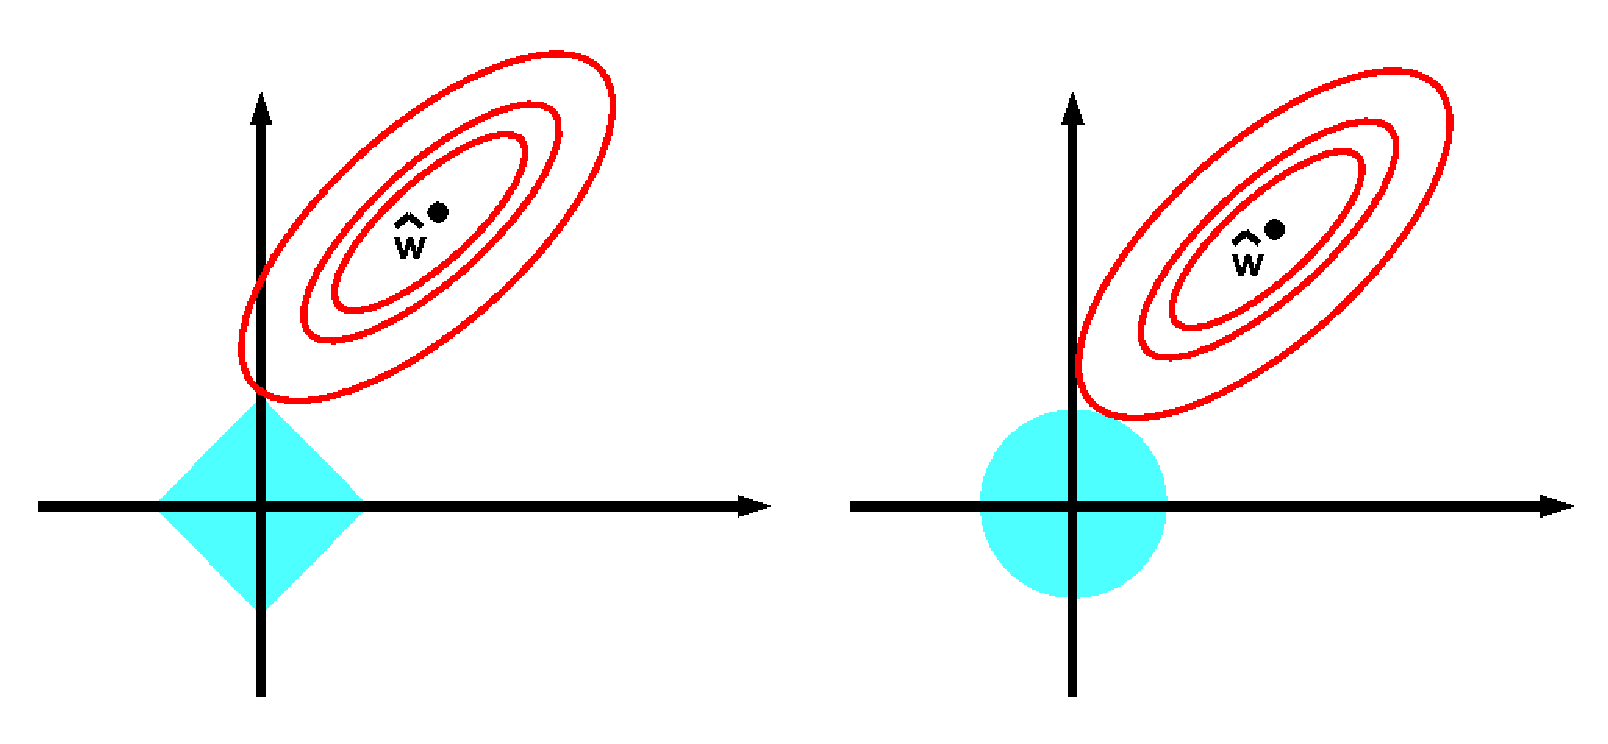
\includegraphics[width=0.5\textwidth]{L2L1contours}
\caption{Illustration of $\ell_1$ (left) vs $\ell_2$ (right) regularization of a least squares problem. Based on Figure 3.12 of (Hastie et al. 2001).}
\end{figure}    
\end{frame}

\begin{frame}{Regularization path}
\begin{itemize}\itemsep=6pt
    \item \textbf{Regularization path}: as we increase $\lambda$, the solution vector $\hat{\bm{w}}(\lambda)$ will tend to get sparser, although not necessarily monotonically. We can plot the values $\hat{w_j}(\lambda)$ vs $\lambda$ for each feature $j$.
    \item \textbf{Ridge regression}: for any finite value of $\lambda$, all coefficients are non-zero; furthermore, they increase in magnitude as $\lambda$ is decreased.
    \item \textbf{Lasso}: as $B$ increases, the coefficients gradually ``turn on". But for any value between $0$ and $B_{\text{max}} = \|\hat{\bm{w}}_{OLS}\|_1$, the solution is sparse.
\end{itemize}    
    \begin{figure}
    \centering
    \subfigure[]{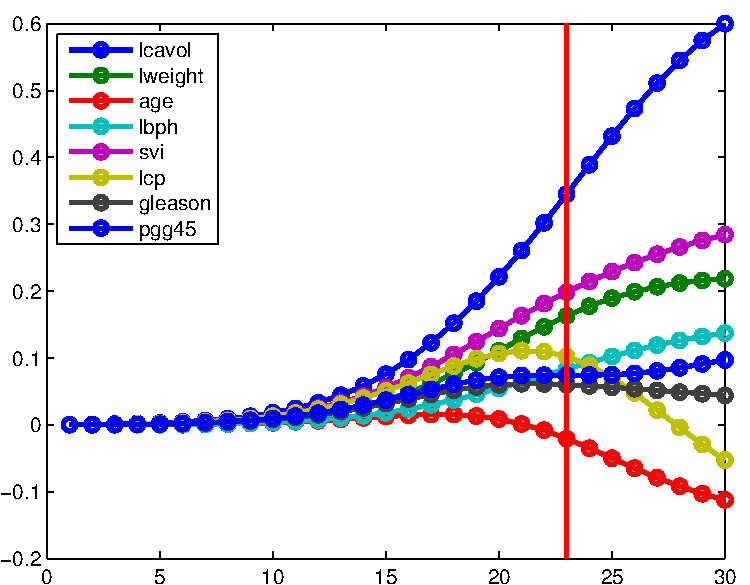
\includegraphics[width=25mm]{ridgePathDemoCv}}
    \subfigure[]{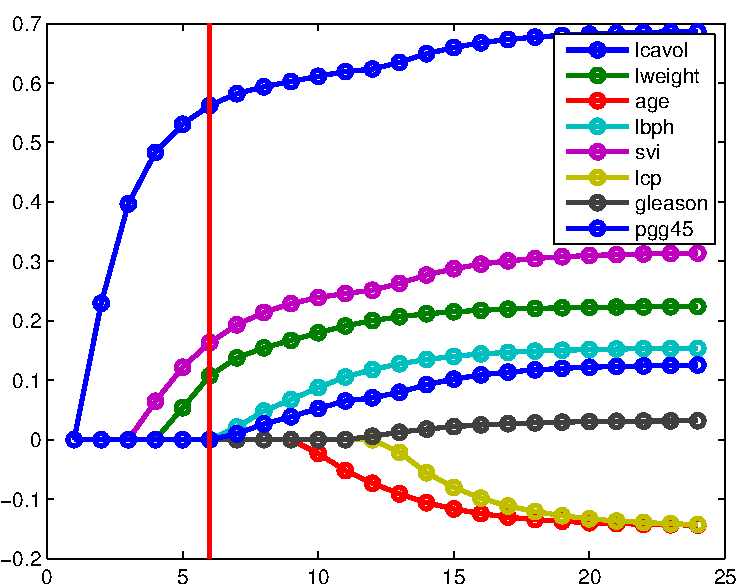
\includegraphics[width=25mm]{lassoPathProstateCv}}
    \caption{(a) Based on Figure 3.8 of (Hastie et al. 2009). Figure generated by \texttt{RidgePathProstate}. (b) Based on Figure 3.10 of (Hastie et al. 2009). Figure generated by \texttt{LassoPathProstate}.}
    \end{figure}    
\end{frame}

\section{$\ell_1$ regularization: algorithms}
\begin{frame}{$\ell_1$ regularization: algorithms\\[-0.3em] 
{\footnotesize \textmd{(See scribes for details)}}}
    \begin{enumerate}
        \item \textbf{Coordinate descent}: optimize variables one by one. We can choose to update the coordinate for which the gradient is steepest.
        \item \textbf{Least-angle regression (LARS)}: similar to forward stepwise regression, but instead of including variables at each step, the estimated parameters are increased in a direction equiangular to each one's correlations with the residual. 
        \item \textbf{Proximal and gradient projection methods}: solve large scale convex optimization problems that has a form
        \begin{equation*}
            f(\bm{\theta}) = L(\bm{\theta}) + R(\bm{\theta})
        \end{equation*}
        where $L(\bm{\theta})$ (loss) is convex and differentiable, and $R(\bm{\theta})$ (regularizer) is convex but not differentiable.
    \end{enumerate}
\end{frame}

\begin{frame}{EM for lasso}
\begin{enumerate}
\setcounter{enumi}{3}
    \item We can solve the lasso problem using \textbf{EM}.
    \begin{itemize}
    \item \textbf{Key:} Use the Laplace distribution as a \textbf{Gaussian scale mixture (GSM)}
    \begin{equation*}
        \text{Lap}(w_j|0,1/\gamma) = \frac{\gamma}{2} e^{-\gamma|w_j|} = \int N(w_j |0, \tau_j^2 ) \text{Ga}(\tau_j^2 |1, \frac{\gamma}{2} )d\tau_j^2
    \end{equation*}
    \item Laplace is a GSM where the mixing distribution on the variances is the exponential distribution.
    \item The corresponding joint distribution has the form
    \begin{equation*}
        \begin{split}
            p(\bm{y},\bm{w},\bm{\tau},\sigma^2|\bm{X}) 
            = & N(\bm{y}|\bm{X}\bm{w},\sigma^2 \bm{I}_N) N(\bm{w}|0,\bm{D}_\tau)\\
              & \text{IG}(\sigma^2|a_\sigma, b_\sigma)[\prod_j\text{Ga}(\tau_j^2|1,\gamma^2/2)]
        \end{split}
    \end{equation*}  
    \end{itemize}
\end{enumerate}
\end{frame}

\begin{frame}{EM for lasso (cont'd)}
\begin{itemize}
    \item In the E step, infer $\tau_j^2$ and $\sigma^2$.
    \item In the M step, estimate $\bm{w}$.
    \item The resulting estimate $\hat{\bm{w}}$ is the same as the lasso estimator.
\end{itemize}

\begin{figure}[h]
\centering
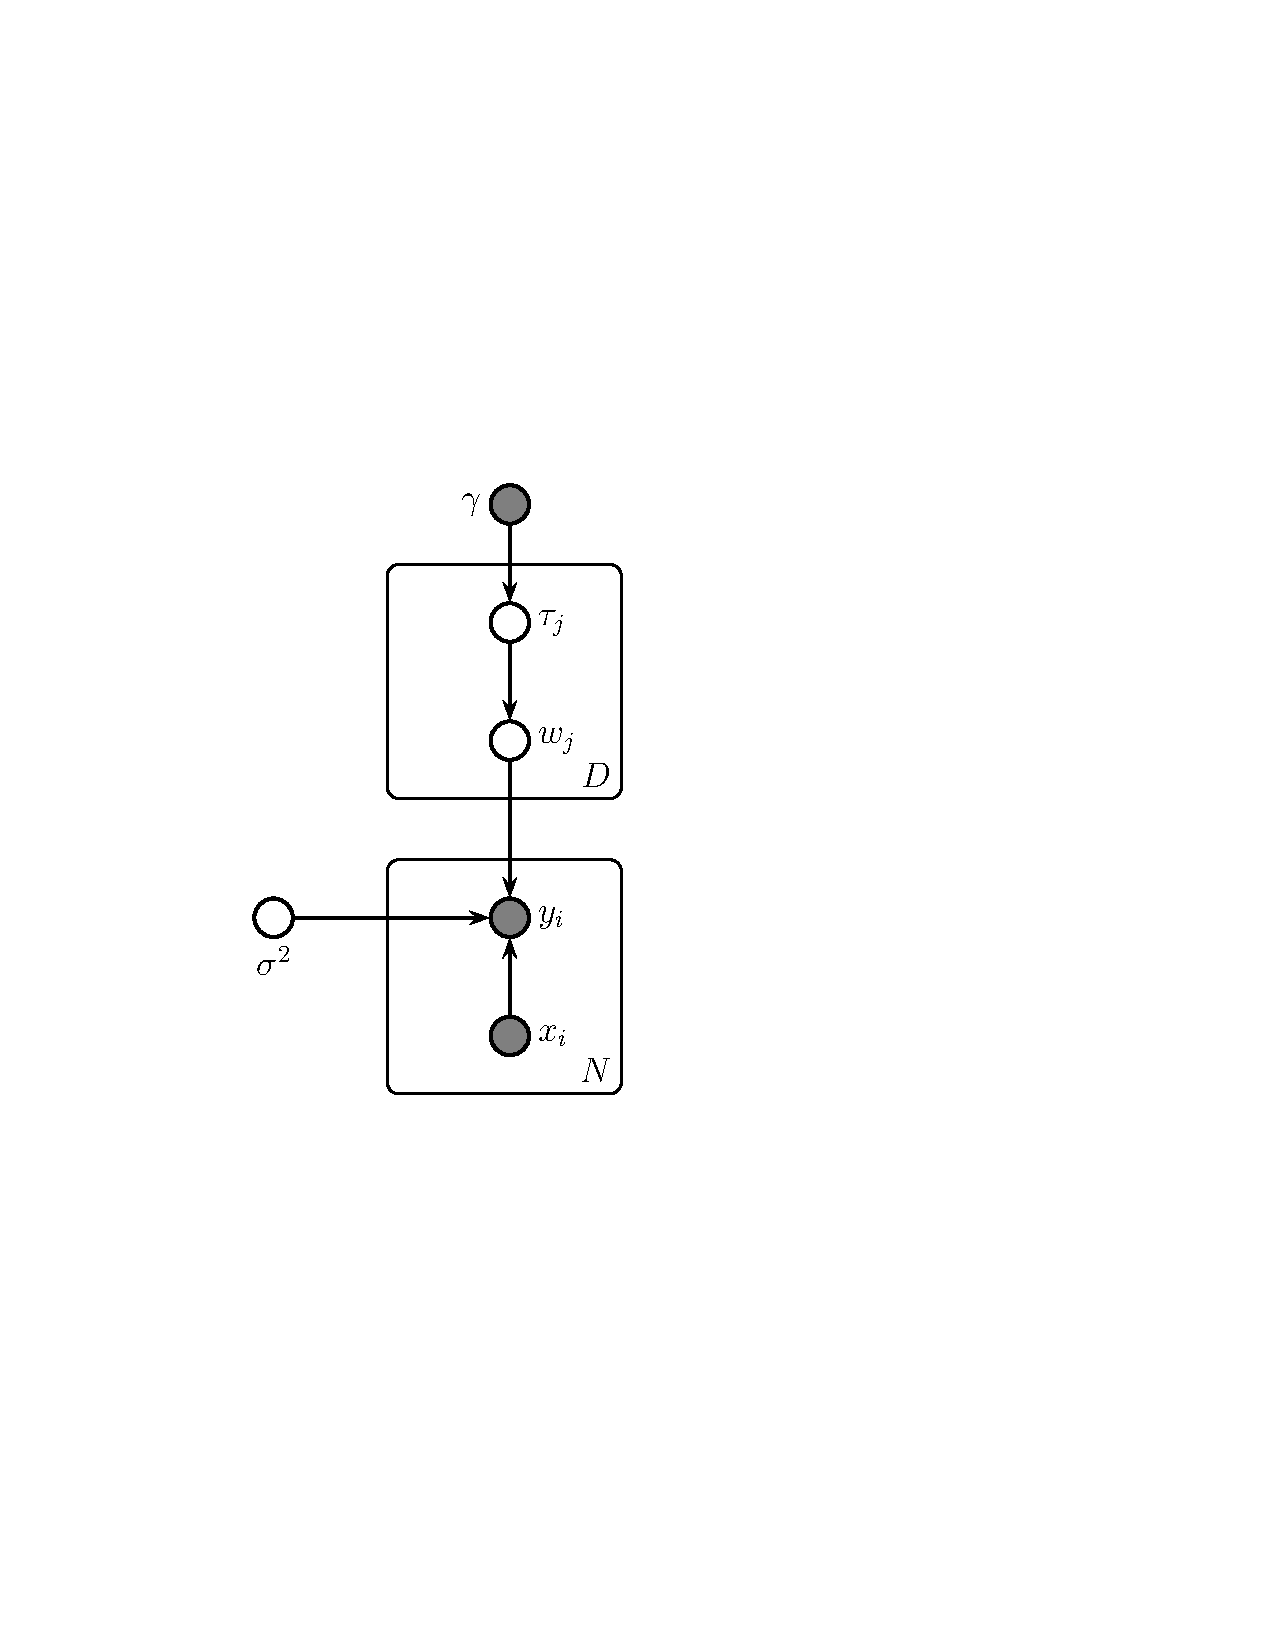
\includegraphics[width=0.3\textwidth]{lassoEMnoSigma}
%\caption*{A figure}
\caption{Representing lasso using a Gaussian scale mixture prior.}
\end{figure}
\end{frame}

\begin{frame}{EM for lasso (cont'd)}
 Why EM?
\begin{itemize}
    \item Can easily derive find $\ell_1$-regularized parameter estimates.
    \item Suggests other priors on the variances besides $\text{Ga}(\tau_j^2|1,\gamma^2/2)$. 
    \item It makes it clear how we can compute the full posterior, $p(\bm{w}|\mathcal{D})$, rather than just a MAP estimate (\textbf{Bayesian lasso}).
\end{itemize}           
\end{frame}

\section{$\ell_1$ regularization: extensions}
\begin{frame}{Group Lasso}
\begin{itemize}
    \item \textbf{Group Lasso} allows predefined groups of covariates to be selected into or out of a model together.
    \item Partition the parameter vector into $G$ groups. We now minimize 
    \begin{equation*}\small
      J(\bm{w}) = \text{NLL}(\bm{w}) + \sum_{g=1}^G \lambda_g\|\bm{w}_g\|_2 \ \ \ \|\bm{w}_g\|_2 = \sqrt{\sum_{j\in g}w_j^2}
    \end{equation*}
    \item E.g. if we have groups $\{1, 2\}$ and $\{3, 4, 5\}$, the objective becomes
    \begin{equation*}\small
      J(\bm{w}) = NLL(\bm{w}) + \lambda \bigg[\sqrt{2}\sqrt{(w_1^2+w_2^2)} + \sqrt{3}\sqrt{(w_3^2+w_4^2+w_5^2)}\bigg] 
    \end{equation*}
    \item Group sparsity: using the square root penalizes the radius of a ball containing the group's weight vector, that is, the only way for the radius to be small is if all elements are small. 
\end{itemize}
\end{frame}    

\begin{frame}{GSM interpretation of group lasso}
\begin{itemize}
    \item Group lasso is equivalent to MAP estimation using the following prior
    \begin{equation*}\small
      p(\bm{w}|\gamma, \sigma^2) \propto \exp(-\frac{\gamma}{\sigma}\sum_{g=1}^G \|\bm{w}_g\|_2)
    \end{equation*}
    \item Now one can show that this prior can be written as a GSM, as follows
    \begin{equation*}\small
        \bm{w}_g|\sigma^2,\tau_g^2 \sim N(0,\sigma^2 \tau_g^2 \bm{I}_{d_g} ) \ \ \tau_g^2|\gamma \sim \text{Ga}(\frac{d_g+1}{2},\frac{\gamma}{2})
    \end{equation*}
    where $d_g$ is the size of group $g$. 
    \item There is one variance term per group, each of which comes from a Gamma prior, whose shape parameter depends on the group size, and whose rate parameter is controlled by $\gamma$.
\end{itemize}
\end{frame}    

\begin{frame}{Sparse group lasso}
\begin{figure}[h]
\centering
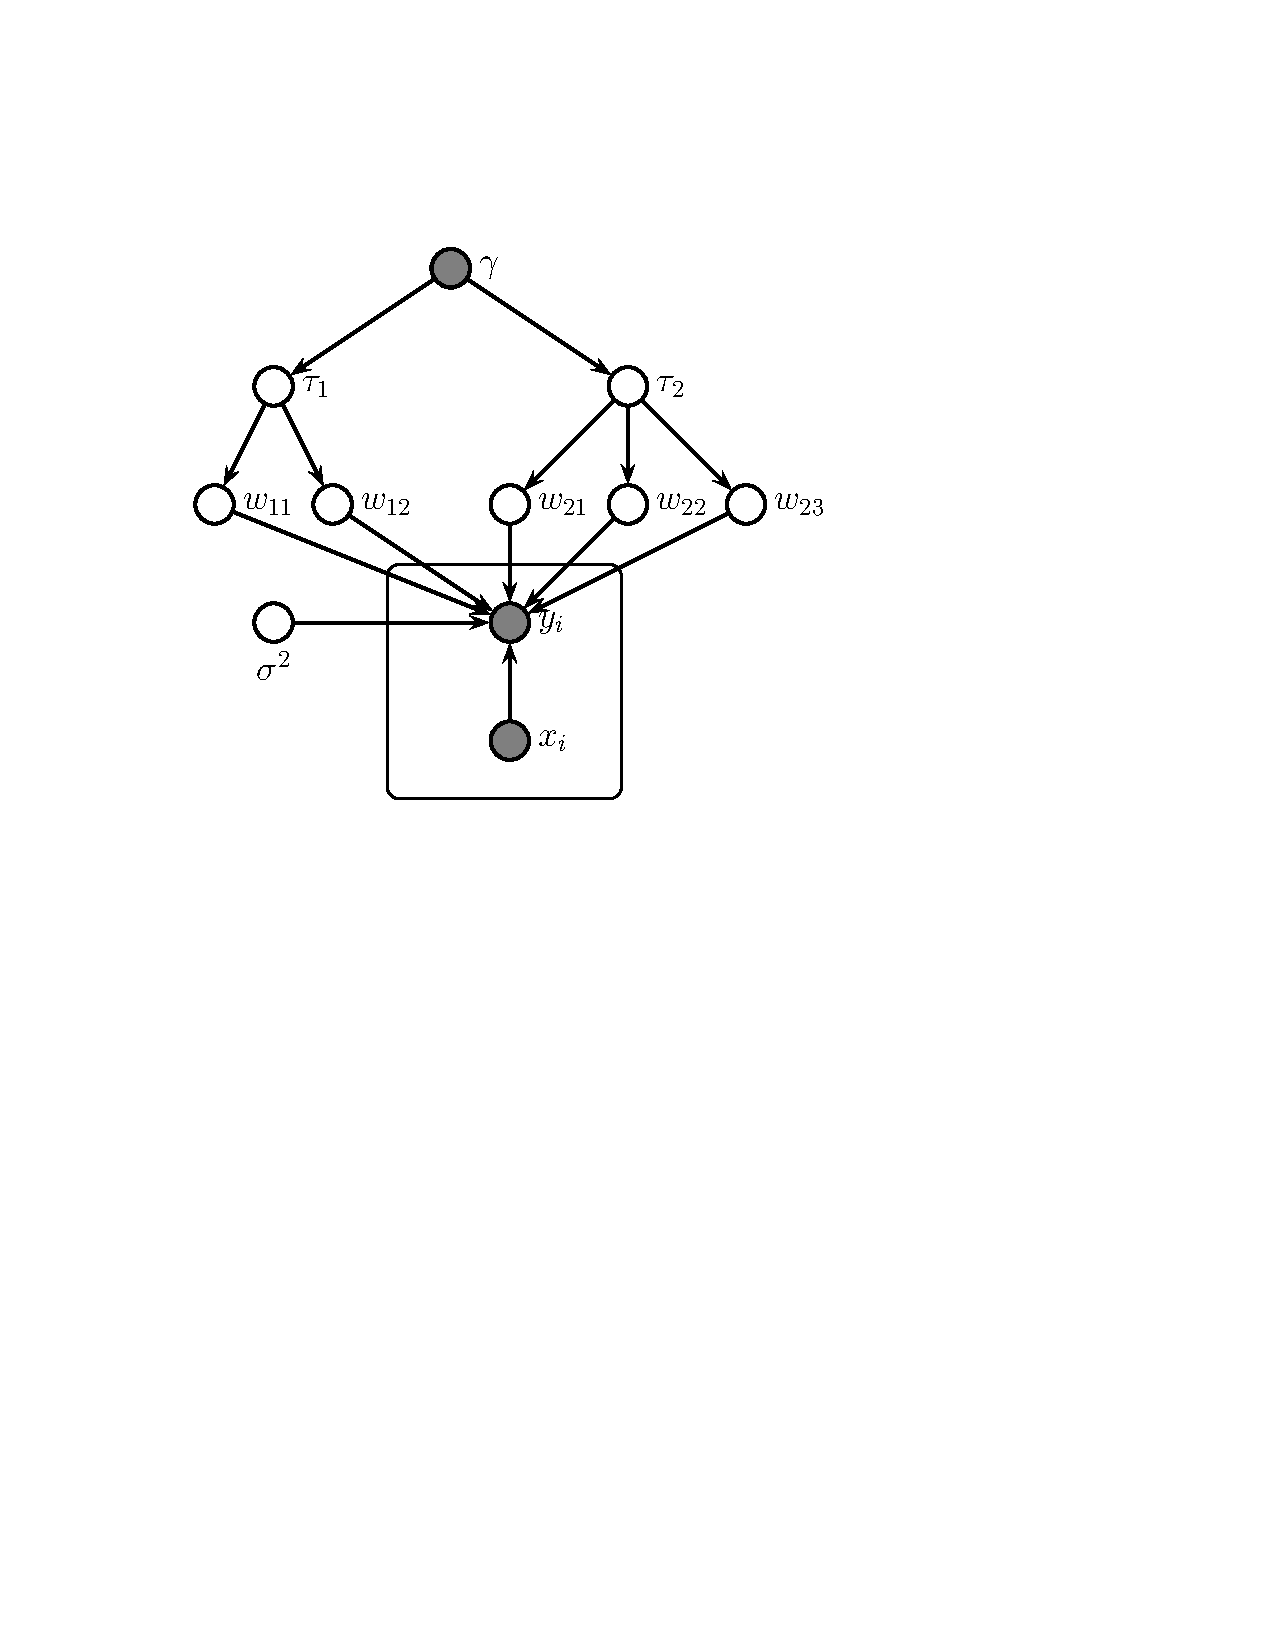
\includegraphics[width=0.35\textwidth]{groupLassoBayesNoSigma}
%\caption*{A figure}
\caption{Graphical model for group lasso with 2 groups, the first has size $G_1 = 2$, the second has size $G_2 = 3$.}
\end{figure} 
\begin{itemize}
    \item The group lasso does not yield sparsity within a group. That is, if a group of parameters is non-zero, they will all be non-zero.
    \item Consider \textbf{sparse group lasso} criterion:
    \begin{equation*}
        J(\bm{w}) = \text{NLL}(\bm{w}) + \lambda_1 \sum_{g=1}^G \|\bm{w}_g\|_2 + \lambda_2 \|\bm{w}_g\|_1
    \end{equation*}
\end{itemize}
\end{frame}

\begin{frame}{Fused lasso}
\begin{itemize}
    \item \textbf{Fused lasso}: we want neighboring coefficients to be similar to each other, in addition to being sparse, by using a prior
    \begin{equation*}
      p(\bm{w}|\sigma^2) \propto \exp(-\frac{\lambda_1}{\sigma}\sum_{j=1}^D|w_j| -\frac{\lambda_2}{\sigma}\sum_{j=1}^{D-1}|w_{j+1}|-w_j)
    \end{equation*}
\end{itemize}
\end{frame}

\section{Non-convex regularizers}
\begin{frame}{Non-convex regularizers}
Potential problems of Laplace prior:
\begin{itemize}
    \item It does not put enough probability mass near $0$, so it does not sufficiently suppress noise.
    \item It does not put enough probability mass on large values, so it causes shrinkage of relevant coefficients, corresponding to ``signal".
\end{itemize}
Solution:
\begin{itemize}
    \item Use more flexible kinds of priors which have a larger spike at $0$ and heavier tails.
\end{itemize}
\end{frame}

\begin{frame}{Generalized Norms: Bridge Regression}
\textbf{Bridge regression} has the form
\begin{equation*}
  \hat{\bm{w}} = \text{NLL}(\bm{w}) + \lambda \sum_j |w_j|^b
\end{equation*}
for $b \geq 0$. This corresponds to MAP estimation using a \textbf{exponential power distribution} given by
\begin{equation*}
  \text{ExpPower}(\bm{w}|\mu,a,b) = \frac{b}{2a\Gamma(1 + 1/b)} \exp(-\frac{|\bm{w}-\mu|^b}{a}) 
\end{equation*}

\begin{itemize}
    \item  Convex objective function (true norm): $b\geq1$.
    \item  Encourages sparse solutions (cusp at zero): $b\leq1$.
    \item  Lasso/Laplacian (convex \& sparsity): $b=1$.
    \item  Ridge/Gaussian (classical, closed form solutions): $b = 2$.
    \item  Sparsity via discrete counts (greedy search): $b \rightarrow 0$.
    \end{itemize}    
\end{frame}

\begin{frame}{Hierarchical adaptive lasso}
\begin{itemize}
    \item Recall: lasso may use a large value of $\lambda$ to ``squash" the irrelevant parameters, but this then over-penalizes the relevant parameters.
    \item Bayesian can associate a different penalty parameter with each parameter.
    \item How? Let $\tau_j^2$ have its own private tuning parameter, $\gamma_j$, which coming from the conjugate prior
    \begin{equation*}
      \begin{split}
          \gamma_j & \sim \text{IG}(a, b)\\
          \tau_j^2|\gamma_j & \sim \text{Ga}(1,\gamma_j^2/2)\\
          w_j|\tau_j^2 & \sim N(0,\tau_j^2)
      \end{split}
    \end{equation*}
\end{itemize}
\end{frame}

\end{document}